\chapter{DUCC Overview}

    \section{What is DUCC?}

    DUCC stands for Distributed Uima Cluster Computing. DUCC is a cluster management system
    providing tooling, management, and scheduling facilities to automate the scale-out of
    applications written to the UIMA framework.

    Core UIMA provides a generalized framework for applications that process unstructured
    information such as human language, but does not provide a scale-out mechanism. UIMAAS provides
    a scale-out mechanism to distribute UIMA pipelines over a cluster of computing resources, but
    does not provide job or cluster management of the resources. DUCC defines a formal job model
    that closely maps to a standard UIMA pipeline. Around this job model DUCC provides cluster
    management services to automate the scale-out of UIMA pipelines over computing clusters.

    \section{DUCC Job Model}

    The DUCC Job model consists of standard UIMA components: a Collection Reader (CR), a CAS Multiplier
    (CM), one or more application Analysis Engines (AE), and a CAS Consumer (CC).  In theory, any
    CR, CM, or CC will work with DUCC, but DUCC is all about scaleout.  In order to achieve good
    scaleout these components must be constructed in a specific way.

    The Collection Reader builds input CASs and forwards them to the UIMA pipelines.  In the DUCC
    model, the CR is run in a process separate from the rest of the pipeline. In all but the smallest
    clusters it is run on a machine that is separate from the rest of the pipeline.  To achieve
    scalability, the CR must create very small CASs that do not contain data, but which contain
    references to data; for instance, file names.  Ideally, the CR should run in a process not much
    larger than the smallest Java virtual machine.  Later sections demonstrate methods for 
    achieving this.

    Each pipeline must contain at least one CAS Multiplier which receives the CASs from the
    CR.  The CMs encapsulate the knowledge of how to recieve the data references in the small
    CASs received from the CRs.  

    DUCC does not provide any mechanism for receiving output CASs.  Each application must
    supply its own CAS Consumer which serializes the output of the Analytic Engines for 
    consumption by other entities (as serialized CASs, perhaps, or as some other form of
    data, depeneing on what the other entities are.).

    A DUCC job therefore consists of a small specification containing the following items:
    
    \begin{itemize}
      \item The name of a file containing the CR descriptor.
      \item The name of a file containing the CM descriptor.
      \item The name of a file containing the AE descriptor.
      \item The name of a file containing the CC descriptor.
      \item Other information required to parameterize the above and identify the job
        such as log directory, working directory, desired scaleout, etc.  These are
        described in detail in subssequent sections.
    \end{itemize}

    On job submission, DUCC examines the job specification and automatically creates and
    a scaled-out UIMA-AS service with a single process executing the CR as a UIMA-AS
    client and and as many processes as possible exeuting the CM, AE, and CC pipeline 
    as UIMA-AS service instances.

    DUCC provides other facilities in support of scaleout of UIMA pipelines:
    \begin{itemize}
      \item The ability to reserve all or part of a node in the cluster.
      \item Automated management of services required in support of jobs.
      \item The ability to schedule and execute arbitrary processes on nodes in the
        cluster.
      \item Debugging tools and support.
      \item A web server to display and manage work and cluster status.
      \item A CLI and a Java API to support the above.
    \end{itemize}
    
    \section{DUCC From UIMA to Full Scaleout}

    In this section we demonstrate the progression of a simple UIMA pipeline to a fully
    scaled-out job running under DUCC.

    \paragraph{UIMA Pipelines}
    The DUCC job model is defined in terms of the UIMA and UIMA-AS framework. A UIMA pipeline
    contains a Collection Reader, one or more Analysis Engines connected in a pipeline, and a CAS
    Consumer as shown in Figure ~\ref{UIMA-pipeline}.

    \begin{figure}[H]
      \centering
      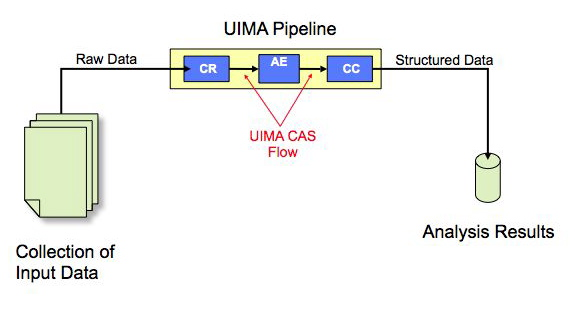
\includegraphics[bb=0 0 575 310, width=5.5in]{images/uima-pipeline.jpg}
      \caption{Standard UIMA Pipeline}
      \label{UIMA-pipeline}
    \end{figure}

    \paragraph{UIMA-AS  Scaled Pipeline}
    With UIMA-AS the CR is separated into a discrete process and a CAS Multiplier is introduced 
    into the analytic pipeline as an interface between the CR and the pipeline, as shown in Figure
    ~\ref{UIMA-AS-pipeline} below.
    Multiple analytic pipelines are serviced by the 
    CR and are scaled-out over a computing cluster. 

    \begin{figure}[H]
      \centering
      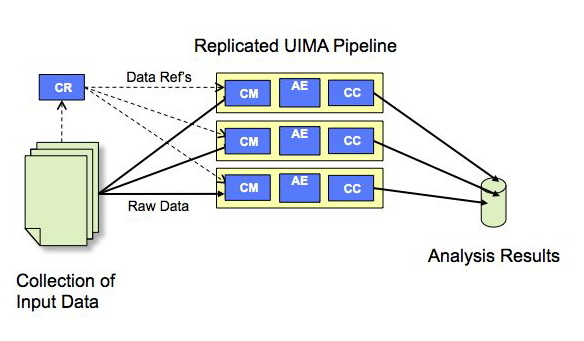
\includegraphics[bb=0 0 584 341, width=5.5in]{images/uima-as-pipeline.jpg}
      \caption{UIMA Pipeline As Scaled by UIMA-AS}
      \label{UIMA-AS-pipeline}
    \end{figure}

    \paragraph{UIMA-AS Pipeline Scaled By Ducc}
    Under DUCC, the Collection Reader is executed in a process called the Job Driver (or JD). The 
    analytic pipelines are executed in one or more processes called Job Processes (or JPs). The JD 
    process provides a thin wrapper over the CR to enable communication with DUCC and to direct 
    CASs to the JPs. Similarly the JP provides a thin wrapper over the analytics as shown in Figure 
    ~\ref{UIMA-AS-pipeline-DUCC} below.

    \begin{figure}[H]
      \centering
      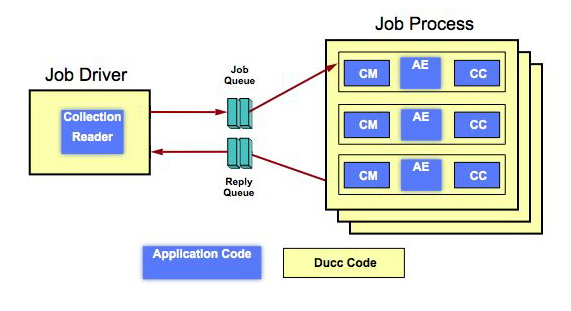
\includegraphics[bb=0 0 571 311, width=5.5in]{images/ducc-sequential.jpg}
      \caption{UIMA Pipeline As Automatically Scaled Out By DUCC}
      \label{UIMA-AS-pipeline-DUCC}
    \end{figure}

    \paragraph{UIMA-AS Pipeline with User-Supplied DD Scaled By DUCC}
    On job submission, the DUCC CLI inspects the XML defining the analytic and generates a UIMAAS
    Deployment Descriptor (DD) from it. DUCC generates job-unique queue endpoints, sets up the
    queues, and sets up multiple pipeline threads so that the entire transformation from the user's
    core-UIMA job to full UIMA-AS scalout is transparent and automatic.  A simple collection of
    parameters, known as the Job Specification (essentially a Java properties file) defines the CR,
    CM, AE, and CC, threading level, logging parameters, etc. Taken together the Job Descriptor, Job
    Driver, and set of Job Processes comprise a DUCC job.

    Users may want to provide their own DDs to more fully control the pipeline in the JPs. This
    model is also support by DUCC as in Figure ~\ref{UIMA-AS-pipeline-DUCC-DD}


    \begin{figure}[H]
      \centering
      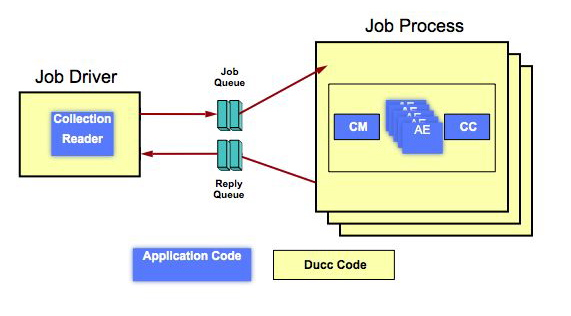
\includegraphics[bb=0 0 571 316,width=5.5in]{images/ducc-parallel.jpg}
      \caption{UIMA Pipeline With User-Supplied DD as Automatically Scaled Out By DUCC}
      \label{UIMA-AS-pipeline-DUCC-DD}
    \end{figure}


    \paragraph{The DUCC Job Descriptor}
    The DUCC Job Descriptor includes properties to enable automated management and scale-out 
    over large computing clusters. Such management includes multiple-user support (jobs run under 
    the identity of the submitting user), a fair-share scheduler capable of balancing resources among 
    all users, automated performance monitoring via the UIMA-AS monitoring facilities, display of 
    job status and performance statistics via a built-in web server, and error-handling of the UIMA 
    pipelines, also using the UIMA-AS facilities. 

    \paragraph{DUCC Command-Line Interface}
    DUCC provides a Command Line Interface (CLI) to submit UIMA pipelines for execution as jobs. 
    (An Application Programming Interface (API) is in progress but not available with the current 
    release.) The CLI inspects the pipeline XML descriptors (as named in the Job Specification) 
    and automatically generates UIMA-AS Deployment Descriptors. The descriptors are passed to 
    the DUCC orchestration tools which establish the Collection Reader inside a Job Driver (JD) 
    process as a UIMA-AS service client. The Job Specification is given to the Resource Manager 
    which returns the identities of the nodes where the JPs (Job Processes) are to be run. Finally the 
    JPs are started with the pipeline's AEs as UIMA-AS services and the JD starts the CR which begins 
    delivering CASs. Endpoint management, creation of the DD, spawning and management of the CR 
    and AEs are all automated by DUCC. 

    \section{Error Management }
    A classic problem of large distributed systems is error management. Small errors can scale-out
    so that a single typo or oversight can flood the system with redundant error notifications and
    waste significant resources with useless computation. It can also be very difficult to isolate
    errors which can occur anywhere in the network. To manage this process DUCC provides a number of
    features.

    DUCC uses the UIMA-AS error-handling facilities to reflect errors from the JPs to the JDs. The
    JD wrappers implement logic to enforce error thresholds, to log the errors coherently, and to
    inform the web server. All error thresholds are configurable. Additionally, the user may
    implement custom logic to determine whether errors should be considered fatal or transient, and
    the number of failures to tolerate. Each job may provide its own fully customized error handling
    policy.

    A large UIMA application can take significant time initializing, reading from databases, and so
    on. The initialization process itself can be fragile and error-prone. It would be wasteful and
    useless to allow such an application to be scheduled on a large number of cluster nodes only to
    fail. To manage this, DUCC enforces two policies:
    
    \begin{itemize}
        \item JPs are allowed a maximum number of failures in the initialization stage before DUCC
          terminates the job.
 
        \item A minimum number of processes is allocated to a job when it starts. The job is not
          allocated additional processes until at least one JP completes the initialization phase,
          at which point the job becomes eligible for more processes.
    \end{itemize}
    
    Once a JP is initialized the error handling is slightly different. Errors at this stage may be
    transient: network failures, service failures, etc. Or they may be systemic in the application
    (bugs). DUCC allows a maximum number of JP failures after initialization and if the threshold is
    exceeded, the job is terminated. If a process has a failure, the failure is reflected back to
    the Job Driver  and the process is terminated. If the threshold has not yet been exceeded, the Resource
    Manager will allocate space and a new process will be started.

    In all failure scenarios, DUCC attempts to capture the associated stack traces and error
    messages and presents them as links in the job pages from the DUCC web server.

    \section{Cluster and Job Management}
    Distributing work over multiple physical processors on a network can be difficult to manage,
    even for relatively small numbers of processors. DUCC provides extensive tooling manage the
    cluster and the jobs running on it.

    \begin{description}
        \item[Multiple User Support] DUCC runs all work under the identity of the submitting user. This
          provides a level of security and privacy for each user and their job. Logs are written with the
          user's credentials into the user's file space designated at job submission, enabling users to
          manage them as needed.

        \item[Fair-Share Scheduling] DUCC is intended to support UIMA processing of natural
          language.  This work is inherently memory intensive. In order to insure that the pipelines
          execute efficiently, resources need to be allocated according to the amount of real RAM used
          by each pipeline.
          
          To manage this, DUCC contains a scheduler designed to allocate nodes in the cluster according to
          declared memory usage. All RAM is treated as a single, distributed pool of memory. "Fair" share
          means that the memory is allocated such that each user is allocated the same amount regardless
          of the number of jobs the user has submitted. Each user's fair-share is then divided equally
          among all their jobs. Machines are then allocated to jobs so the total memory in the machines
          assigned to a user is the same as their fair-share. Often some users don't need (and can't use)
          their fair share, in which case the DUCC scheduler allocates the lefovers to users that are able
          to use it.
    \end{description}

    The DUCC scheduler provides the ability to "weight" resource requests to provide other than
    a simple fair-share of RAM allocation. There is also a priority scheme that insures some types of
    work are always scheduled irregardless of fair-share considerations. There is also a mechanism
    for partitioning the nodes according to arbitrary constraints ("closeness" to constrained
    resources, priority usage such as "production" vs. "development" use, etc.), and assigning jobs
    to specific partitions or "nodepools".

    DUCC assumes that most jobs written to the UIMA framework are fully parallel and that individual
    processes can be evicted as needed; as well it assumes that process can be added to a job if
    resources are available. The DUCC scheduler uses these properties to dynamically expand or
    reduce the number of processes assigned to jobs, according to fair-share policies and the amount
    of work in the system. For example, if a new user submits a job, this will generally reduce
    everybody's fair-share, and result in some processes being evicted to make room for the new
    user.  Similarly, if all of a user's jobs exit, then the remaining jobs will be allocated the
    resources that are now freed. 

    Some jobs may not be parallel, or for some other reason, cannot tolerate being evicted and
    restarted. The DUCC scheduler implements a policy to allow jobs with "fixed" (or "pinned") node
    allocations whic prevents those jobs from being preempted; conversly the "fixed" policy prevents
    those jobs from growing. Thus, once scheduled, this type of job is "fixed" in place and will
    never move to different nodes.

    The scheduler also supports the concept of Reservations. A reservation has no job associated
    with it; users are allowed to use the reserved resources as they wish (within
    reason). Reservations for full (dedicated) nodes or for partial nodes (based on RAM) are
    supported.

    \begin{description}
      \item[Job Lifetime Management and Orchestration] DUCC includes an orchestrator that manages the
        lifetimes of all jobs, services, and reservations. Jobs are submitted to the orchestrator, which
        is responsible for insuring pre-requisite services are available and that resources are
        scheduled for the job. It starts the job's JD and JP processes and signals the JD to start
        servicing work to the JPs. It is also responsible to keep the scheduler and web server apprised
        of the status of all jobs.
        
      \item[DUCC Agents] A process called the DUCC Agent is run on each node managed by DUCC. This 
        process has several roles: 
        \begin{itemize}
            \item Manage JP and JD processes. The agent starts, stop, and manages the life cycle of these
              processes. It also monitors performance statistics on behalf of these processes, reporting to
              the web server.
 
            \item Monitor node performance and "aliveness". The agent monitors CPU, memory, etc, and provides the
              information in regular heartbeats that are watched by the Resource Manager and Web server for
              scheduling and reporting purposes.
            
            \item Watch for rogue processes. The agents watch for processes not associated with DUCC jobs or other
              DUCC-initiated work and reports to the web server. Administrators are then able to easily
              identify and reap processes that may be interfering with DUCC jobs.  
        \end{itemize}

        \item[DUCC Web server] DUCC  provides a web server displaying all aspects of the system:
          \begin{itemize}
              \item All jobs in the system with relevant information: user, times, work finished work completed,
                processes allocated, and many other. For each job, additional pages provide details including
                node, PID, stat status of all work items, the submitted job specification, etc. If errors occur,
                links from the job entry to the errors in the logs are provided.
                
              \item All reserved nodes with relevant information: user, times, nodes, processes running in the
                reservation, etc.
                
              \item All nodes in the system and their status, usage, etc. 
                
              \item All services and rel-event information: user, nodes, usage, who is using the
                services, queue size, etc.
                
              \item The status of all DUCC management processes.  
          \end{itemize}


        \item[Management Scripting] DUCC provides rich scripting support to:
          \begin{itemize}
              \item Start and stop full DUCC systems.
 
              \item Start and stop and individual DUCC components.
 
              \item Add and delete nodes from the DUCC system.
 
              \item Discover DUCC processes (e.g. after partial failures).
 
              \item Find and kill errant job processes belonging to individual users.
          \end{itemize}
      \end{description}

      \section{Service Management}
      \paragraph{Overview.} 
      Services, in the context of DUCC, are long-running processes that await requests from
      UIMA pipeline components and return something in response. Services can be any arbitrary process
      using any arbitrary communication protocol but in the current version of DUCC only UIMA-AS
      services are fully supported.

      The DUCC service manager implements several high-level functions:
      
      Insure services are available for jobs before allowing the jobs to start. This fail-fast
      prevents unncessary allocation of resources (with potential eviction of healthy processes) for
      jobs that can't run, as well as quick feedback to users that something is amis.
      
      Automate the startup, care, and management of services.
      
      Report on the state of services: processes, queue depths, comsumers, and so on.  

      \paragraph{Service Types.}
      DUCC supports two types of services: UIMA-AS and CUSTOM:
      
      \begin{description}
          \item[UIMA-AS] This is a "normal" UIMA-AS service. DUCC fully supports all aspects of UIMA-AS
            services.
            
          \item[CUSTOM] This is any arbitrary service. DUCC supports monitoring of CUSTOM services
            and performs job dependency checks, but (in the current version) does not support start
            and stop of CUSTOM services.
      \end{description}

      \paragraph{Service Endpoints.} Services are referenced by a specifier called a service
      endpoint.. The service endpoint is a formatted string indicating:

      \begin{itemize}
         \item The service type: UIMA-AS or CUSTOM.

         \item The service name. For UIMA-AS services, this is the name of the queue in the ActiveMq
           Broker used for communication with the service. For CUSTOM services this is any arbitrary
           string as dictated by the service. Service names must be unique within the system.

         \item For UIMA-AS services only, the URL of the ActiveMq broker.  
      \end{itemize}

      \paragraph{Dependent and Pre-Requisite Services and Jobs.} A {\em dependent service} is a
      service which is dependent on at least one other service to perform it's function. A {\em
        dependent job} is a job which is dependent on at least one service to perform it's function.

      An {\em independent service} service is a service which is required by another job or
      service. (Note that there are no independent jobs.)

      \paragraph{Service Classes.} Services may be started externally to DUCC, explicitly through
      DUCC as a job, or as registered services. These form three natural classes of services with
      slightly different management characteristics.

      \paragraph{Implicit Services.} An implicit service is started externally to DUCC and discovered by DUCC only
      when it is referenced by a job's service-dependency parameter. On submission of a job with a
      dependency on an implicit service, the SM sets up a "ping" thread that check if the service
      exists at the endpoint. If so, the SM adds the service to its list of known services and marks
      the job "ready to schedule". If the service is a UIMA-AS service the SM establishes a monitor
      thread on the queue for reporting purposes. The service is monitored throughout the lifetime of
      the job. If the service should stop responding, its state is updated as "not-responding" but the
      job is allowed to continue as DUCC cannot tell if the job is still using it or not, or if the
      outage is temporary. If the job is a CUSTOM service, the service owner may specifiy custom code
      to run in the ping thread; for CUSTOM services, this same code is used to run both ping and
      monitor functions.
      
      When the job exits, a timer is set and DUCC continues to monitor the service against the
      possibility that subsequent jobs will need it. Once the last job using the service has exited
      and the service timer expired, the SM stops the monitors and purges the service from its
      records.
      
      \paragraph{Submitted Services.} A submitted service is a service that is submitted to DUCC as a job. A
      submitted service is essentially a normal DD-style job (a job in which the user supplies the
      full UIMA-AS DD), but without a Collection Reader. Because DUCC is managing this service it can
      provide more support than for implicit services.
      
      Submitted services can be dependent upon other services. When such a service enters the system,
      DUCC verifies it's pre-requisite services. When (or if) all pre-requisite services are availble
      DUCC marks the new service "ready to schedule". The lifecycle of the service is monitored so
      that dependent services and jobs are marked "ready to schedule" only after the submitted service
      has completed its initialization phase. A ping thread and queue monitor are also started against
      the newly submitted service. If the submitted service is unable to successfully initialize,
      services and jobs that are dependent on it are marked "not runnable" and the DUCC Orchestrator
      cancels them.
      
      DUCC manages the lifecycle of submitted services, but because they are submitted by entities
      other than DUCC, the SM performs no additional management for them. When a submitted service is
      canceled by its owner, DUCC stops the ping and queue monitors. Any jobs or services dependent on
      it are allowed to continue until they complete or fail due to unavailability of the service.
      
      \paragraph{Registered Services.} Registered services are fully managed by DUCC. A service is
      registered with DUCC using the CLI to provide the full job specification of the service, the
      initial number of instances of the service, and whether the service should be automatically
      started when DUCC itself is started. Registered services started when DUCC is started are
      called automatic services.  Registered services that are started only when referenced by other
      dependent jobs or services are called on-demand services. The service is registered with the
      submitter's credentials and is run with that user's credentials when it is started.

      \todo Fix and properly place this paragraph.
          Ping and monitor threads are started. Jobs and other services may use these services in the same
          manner as submitted services. If an automatic service instance should die or be canceled out of
          the scope of the SM, the SM will restart the instance, maintaining the registered number of
          instances at all time. Automatic services are not terminated when their dependent jobs/services
          exit; they're termanted only when DUCC itself is terminated, or by use of the service stop
          command.

      There are several subclasses of Registered Services:
      \begin{description}

        \item[Automatic Services] An automatic service is a registered service that is flagged to be
          automatically started when the DUCC system is started. When DUCC is started, the SM checks the
          service registry for all service that are marked for automatic startup. The SM submits the
          registered service specification on behalf of its owner. Each such submission is for a single
          service instance.  If found, the SM repeatedly submits the specification until the registered
          number of instances is reached.
          
        \item[On-Demand Services] An on-demand service is a registered service that is started only when
          referenced by the service-dependency of another job or service. f the service is already
          started, the dependent job/service is marked ready to schedule as indicated above. If not, the
          service registry is checked and if a start-on-demand service with an endpoint matching the
          service-dependency is found, DUCC submits the service on behalf of the service owner (in the
          same manner as for automatic servic establishing the registered number of service instances, a
          ping thread, and a monitor). When the service has completed initialization the dependent
          job/service is marked ready to schedule. If the on-demand service cannot be found in the
          registery, the referring entity is marked not-startable and the DUCC Orchestrator cancels it.
          
          Subsequent jobs and services that reference the on-demand service will use the started
          instances.  When the last job/service that references the on-demand service exits, a
          (configurable) timer is established to keep the service alive for a while (in anticipation that
          it will be needed again soon.)  When the keep-alive timer exipires, and there are no more
          dependent jobs/services, the on-demand service is automatically stopped to free up its resources
          for other work.

          \item[External Services] External services consist of only a ping thread.  The service
            itself is not managed in any way by DUCC.  This is useful for managing dependencies
            on services that are not under DUCC control: DUCC can detect and report on the health
            of these services and take appropriate actions on dependent jobs if the services
            are not responsive.
      \end{description}
          
    \paragraph{Registered Service Management.} The CLI for registered services provides several functions:

    \begin{description}
        \item[Register] Register files a service specification with the SM. The service may optionally
          be started as part of registration. The service definition and state is persisted over system
          restarts and is deleted only with the Unregister function.
          
        \item[Unregister] Unregister removes the service specification. The service is stopped if it is
          started and not busy. (Note that if the service is busy, jobs and services that are dependent
          on it may subsequently fail.)
          
        \item[Modify] Modify allows dynamic update of some parameters of registered services:
            \begin{itemize}
              \item Automatic and On-Demand state.
              \item The minimum number of service instances to start when the service is started.  
            \end{itemize}

        \item[Start] Start submits the service specification to the DUCC Orchestrator (repeatedly,
          until the correct number of instances are started). If the service is explicitly started
          with the start CLI, the service continues to run even after the last reference is gone,
          regardless of whether it is automatic or on-demand. Start is also used to increase the
          number of running instances of a service. The registry may be optionally updated to
          reflect the new number of started instances.
          
        \item[Stop] Stop stops the instances for a registered service. The registry may be
          optionally updated to reflect the new number of instances that are still running.

        \item[Query] A CLI-based query is supplied to report on all services known to DUCC, their
          states, their instances, their dependent jobs, and performance statistics for the service.
    \end{description}
        
